
\documentclass[10pt,conference]{IEEEtran}
\usepackage[utf8]{inputenc}
\usepackage[T1]{fontenc}
\usepackage{amsmath,amssymb}
\usepackage{graphicx}
\usepackage{booktabs}
\usepackage{multirow}
\usepackage{array}
\usepackage{url}
\usepackage[hidelinks]{hyperref}
\setlength{\textfloatsep}{4pt plus 1pt minus 1pt}
\setlength{\floatsep}{4pt plus 1pt minus 1pt}
\setlength{\intextsep}{5pt plus 1pt minus 1pt}
\setlength{\abovecaptionskip}{3pt}
\setlength{\belowcaptionskip}{0pt}
\renewcommand{\arraystretch}{0.94}
\setlength{\parskip}{0pt}
\hyphenpenalty=1000
\sloppy
\begin{document}
\title{\vspace{-1.2em}\normalsize THE UNIVERSITY OF LAHORE $\bullet$ DEPARTMENT OF INTELLIGENT SYSTEMS $\bullet$ AI-101\\[2pt]
\Large Task C3: Image Captioning with a CNN Encoder and an LSTM Decoder}
\author{\normalsize Rizwan Ali \quad|\quad Roll No.\ 70177926 \quad|\quad Section C\\
\normalsize\url{https://github.com/RaeesRizwan09/AI101-ML-Assignment-70177926} \quad|\quad Instructor: Dr.\ Muhammad Awais, AI Architect}
\maketitle
\vspace{-1.4em}
\begin{center}\small\itshape A frozen ResNet-50 with a trained attention LSTM decoder reaches corpus BLEU-4 0.227 on 1,091 unseen images. Replacing each image's features with another image's raises validation loss from 2.72 to 3.99 nats, so the decoder is reading the picture and not just the corpus.\end{center}
\vspace{-0.6em}

\section{Introduction}
Describing an image in one sentence couples two hard problems: deciding \emph{what} is in the
picture, and deciding \emph{how} to say it. Flickr8k was built for exactly this
setting~\cite{flickr}: 8,091 photographs, each described independently by five
people. The task is a sequence-to-sequence problem whose source is an image: a convolutional
network compresses the picture into features and a recurrent network writes the caption one token
at a time. The metric (BLEU) rewards \emph{agreement with five annotators}, not truth, so a
caption that is safe and generic can outscore a precise one; separating the two is what the
analysis below does.

\section{Problem Statement}
An image $I$ is mapped to a caption $c=(c_1,\dots,c_T)$, $c_t\in\mathcal{V}$. With a frozen
encoder $E$, we learn
$p_\theta(c\mid I)=\prod_t p_\theta(c_t\mid c_{<t}, E(I))$ by minimising the token-level
cross-entropy
$\mathcal{L}=-\sum_t \log p_\theta(c_t\mid c_{<t},E(I))$ over the training captions.
Two decoders are compared under identical conditions: a \emph{merge} decoder that fuses one
global image vector with the LSTM state, and an \emph{attention} decoder that attends over a
$7\times7$ grid at every step. Both are decoded greedily and with beam search ($k=3,5$) and scored
with corpus BLEU-1\ldots4 against \emph{all five} references. Success is a BLEU-4 well above what a
caption prior alone could reach, a control showing that the decoder's output really depends on the
image, and a qualitative error analysis that says where the remaining gap is.

\section{Dataset Used}
Flickr8k~\cite{flickr} (Kaggle release \path{adityajn105/flickr8k}), obtained from a Hugging
Face mirror so that no Kaggle credentials are needed. It contains 8,091 images and
40,455 captions, five per image, written by human annotators. I split by
\textbf{image} into 6,000 /
1,000 / 1,091: splitting by caption would put four references of an image in
training and the fifth in test, and the test score would measure memorisation. Captions were
lowercased and stripped of punctuation; \texttt{<start>}/\texttt{<end>} delimit them and rare
words become \texttt{<unk>}.

\section{Dataset Statistics}

\begin{table}[t]
\centering
\caption{Flickr8k statistics after preprocessing. The split is by image, the vocabulary is built from training captions only.}
\label{tab:stats}
\scriptsize
\begin{tabular}{l@{\hspace{2pt}}l@{\hspace{5pt}}l@{\hspace{2pt}}l}
\toprule
Property & Value & Property & Value \\
\midrule
Images & 8,091 & Captions & 40,455 (5 each) \\
Train/val/test & 6,000 / 1,000 / 1,091 & Vocabulary & 2,556 words \\
Caption length & mean 10.8, p95 18 & Types before & 7,470 \\
Steps capped at & 22 tokens & Kept at $\geq5$ & 34\% of types \\
OOV, val / test & 3.06\% / 3.03\% & Top word & \texttt{a} (46,730) \\
\bottomrule
\end{tabular}
\end{table}


\section{Methodology}
\subsection{Learning setting}
An encoder--decoder trained by teacher forcing. The encoder is an ImageNet-pretrained
ResNet-50~\cite{resnet} with all weights frozen; its 2,048-d average-pooled vector (or
its 7$\times$7$\times$2048 feature map) is the only visual
input. Freezing is deliberate: fine-tuning 23 M convolutional parameters on 6,000
images on a CPU was out of budget and would overfit. Features were extracted once and cached, so
both decoders see the \emph{same} visual representation and any difference is attributable to the
decoder.

\subsection{Data-split approach}
6,000/1,000/1,091 images, seeded, split on identifiers so that all
five captions of an image stay together. The vocabulary is built from training captions only
(2,556 words kept at frequency $\geq5$), leaving 3.06\,\%
and 3.03\,\% out-of-vocabulary words on validation and test that the model can
never produce. Each training epoch samples one caption per image, so all 6,000 images are
seen every epoch while the five references rotate; validation loss uses all five. Training runs for
50 epochs (9.0 min) for the merge decoder and 30 epochs (33.8 min) for attention with early stopping (patience 6) on validation loss, keeping the best-validation checkpoint.
Every caption is paired with its own image's cached features, and the notebook asserts that mapping
and reports a shuffled-feature control in the Results.

\subsection{Parameter settings}
Embeddings and LSTM hidden states are 256-d in the merge decoder and 512-d with a 256-d attention
space in the attention decoder; dropout 0.5; Adam at $10^{-3}$ with a $\times 0.5$ schedule when
validation loss stalls; gradient norm clipped at 5; batch size 128. Training ran on
\textbf{Intel(R) Core(TM) i5-8265U CPU @ 1.60GHz}, 8 threads, no GPU; feature extraction took
17.7 min (7.6 images/s), and the two
trainings took the times given above. Beam search keeps 3 or 5 hypotheses and applies the length
penalty $\ell^{-0.7}$; without it beam search prefers short captions, since every extra token adds
a negative log-probability.

\section{Results and Analysis}
\subsection{Results}

\begin{table}[t]
\centering
\caption{B1--B4 are corpus BLEU-1\ldots4 against all five references on 1,091 test images; Words counts distinct words over the generated captions and Len is the mean caption length. Clipped n-gram counts and a brevity penalty; checked against \texttt{nltk.corpus\_bleu} (difference $<10^{-6}$).}
\label{tab:bleu}
\scriptsize
\begin{tabular}{l@{\hspace{3pt}}l@{\hspace{5pt}}c@{\hspace{3pt}}c@{\hspace{3pt}}c@{\hspace{3pt}}c@{\hspace{5pt}}c@{\hspace{3pt}}c}
\toprule
Model & Search & B1 & B2 & B3 & B4 & Words & Len \\
\midrule
merge & greedy & 0.557 & 0.380 & 0.248 & 0.163 & 247 & 11.2 \\
merge & beam $k{=}3$ & 0.593 & 0.412 & 0.283 & 0.193 & 253 & 11.2 \\
merge & beam $k{=}5$ & 0.605 & 0.423 & 0.293 & 0.202 & 254 & 10.8 \\
attention & greedy & 0.603 & 0.423 & 0.287 & 0.190 & 311 & 9.9 \\
attention & beam $k{=}3$ & 0.633 & 0.451 & 0.315 & 0.216 & 304 & 9.8 \\
attention & beam $k{=}5$ & 0.640 & 0.461 & 0.326 & \textbf{0.227} & 296 & 9.7 \\
\bottomrule
\end{tabular}
\end{table}



\begin{figure}[t]
\centering
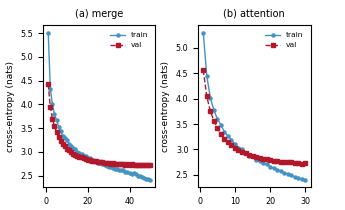
\includegraphics[width=\columnwidth]{figures/C3_fig2_loss.png}
\caption{Training and validation cross-entropy per epoch for both decoders. The gap that opens between the two curves is the overfitting that the best-validation checkpoint protects against.}
\label{fig:loss}
\end{figure}


Attention decoding (beam5) is the best configuration at
BLEU-4 0.227; the merge decoder's best is
0.202.

\textbf{Does the decoder use the image?} Scoring the validation captions twice with the trained
attention decoder -- once with each image's own features, once with another validation image's --
gives 2.72 and 3.99 nats per token (+1.27);
the merge decoder shows the same pattern (2.71 $\rightarrow$
3.70). A decoder that ignored the picture would score the same either way, so
the BLEU above comes from vision and not from the caption prior alone.


\begin{figure}[t]
\centering
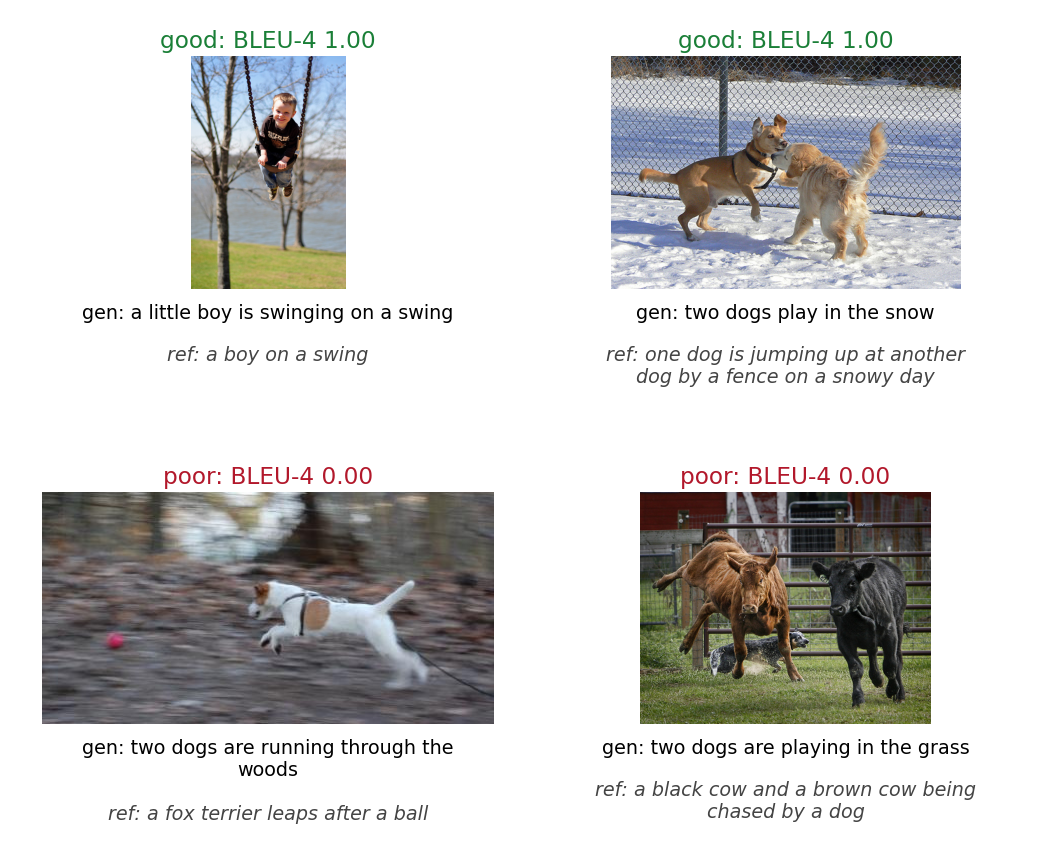
\includegraphics[width=\columnwidth]{figures/C3_fig3_examples.png}
\caption{Generated captions for four test images (best configuration: beam5). Top row: the two highest per-image BLEU-4. Bottom row: the two lowest.}
\label{fig:ex}
\end{figure}


\subsection{Analysis}
\textbf{Does beam search help?} Yes, but the gain is small.
The best beam result is +0.0373 BLEU-4 over greedy. For the merge decoder BLEU-4 moves
0.163 (greedy) $\rightarrow$ 0.193 ($k{=}3$) $\rightarrow$ 0.202 ($k{=}5$);
for attention, 0.190 $\rightarrow$ 0.216 $\rightarrow$ 0.227. Beam search
maximises the sequence log-probability, so it prefers phrases the corpus makes likely. Its risk is
that it replaces a specific word with a more frequent one, so part of the gain can be fluency
rather than accuracy.

\textbf{Generic captions and the distinct-word count.} Beam search does not simply widen the vocabulary: merge moves from 247 distinct words with greedy to 254 at $k{=}5$, attention from 311 to 296, out of 2,556. Attention's extra BLEU is therefore partly template -- fewer words, higher score -- while merge buys its gain without narrowing, so the effect is not a law. Per-token maximum likelihood makes "a dog is running through the grass" the safest continuation for many dog images, and nothing in the objective rewards naming \emph{this} colour or \emph{this} count.

\textbf{Error types.} The poor examples in Fig.~\ref{fig:ex} show counting and identity errors:
one dog becomes two, cows become dogs. Elsewhere the failures are \emph{colour} (a global
average-pooled vector and a $7\times7$ grid both blur it) and \emph{action} (a frozen ImageNet
classifier encodes \emph{what} is present better than \emph{what is happening}). When the image
is ambiguous it falls back on the most frequent people-phrase in Flickr8k, which is why a
captioner needs human review.

\textbf{Merge versus attention.} Attention wins by 0.025 BLEU-4. At each step the decoder can look at one region, so nouns are anchored to the right object even when the phrasing is generic. The merge decoder compresses the whole image into one 256-d vector before the first word is written, which is where its colour and counting errors come from. The two criteria disagree, though: merge has the lower validation loss (2.714 vs 2.723) and the lower BLEU, because per-token likelihood and corpus BLEU are different objectives. The price is speed: attention costs
6.3$\times$ per epoch, since it evaluates 49 locations at every one of the
22 steps.

\textbf{Limitations.} BLEU correlates loosely with human judgement, Flickr8k is small, both
models are trained from scratch on CPU, and zero-shot BLIP would almost certainly beat both.

\section{Conclusion}
A frozen ResNet-50 with a trained attention LSTM decoder reaches BLEU-4 0.227, ahead of the merge decoder (0.202) under identical features and splits. Beam search buys 0.0373 BLEU-4 at best, and it narrows the vocabulary. The metric and the objective both reward fluency, so deployment needs a specificity signal, not a bigger beam. Next: attention maps, a tuned length penalty, and a zero-shot BLIP comparison.

\newpage
\section*{AI Use Disclosure}
I used Claude (Anthropic) as an AI assistant for scaffolding this notebook and drafting report
prose from the numbers it produced. The following parts were generated or substantially assisted by
AI: the notebook's cell structure, the PyTorch training loop, the beam-search and BLEU
implementations, the plotting code and the first draft of Sections I--VII. I verified the content by
re-running the notebook end to end on CPU (hardware and wall-clock time are reported above),
checking that the split is made by image so no caption leaks, that the vocabulary is built from
training captions only, that every caption is paired with its own image's features (asserted in the
notebook, and tested by a shuffled-feature control), and that all five references are passed to the
BLEU scorer -- which I also cross-checked against \texttt{nltk.corpus\_bleu}. All experiments,
results and analysis in this report were produced and checked by me, and I take full responsibility
for this work.

\begin{thebibliography}{9}
\bibitem{flickr} M.~Hodosh, P.~Young, and J.~Hockenmaier, ``Framing image description as a
ranking task: Data, models and evaluation metrics,'' \emph{JAIR}, vol.~47, pp.~853--899, 2013.
\bibitem{resnet} K.~He, X.~Zhang, S.~Ren, and J.~Sun, ``Deep residual learning for image
recognition,'' in \emph{CVPR}, 2016.
\bibitem{showtell} O.~Vinyals, A.~Toshev, S.~Bengio, and D.~Erhan, ``Show and tell: A neural image
caption generator,'' in \emph{CVPR}, 2015.
\bibitem{attn} K.~Xu \emph{et al.}, ``Show, attend and tell: Neural image caption generation with
visual attention,'' in \emph{ICML}, 2015.
\bibitem{karpathy} A.~Karpathy and L.~Fei-Fei, ``Deep visual-semantic alignments for generating
image descriptions,'' in \emph{CVPR}, 2015.
\end{thebibliography}
\end{document}
